\documentclass[preprint,12pt]{elsarticle}
\usepackage{amsmath,amssymb}
\usepackage{graphicx}
\usepackage{booktabs}
\usepackage{tabularx}
\usepackage{longtable}
\usepackage{url}
\def\UrlBreaks{\do\/\do\-\do\:\do\a\do\b\do\c\do\d\do\e\do\f\do\0\do\1\do\2\do\3\do\4\do\5\do\6\do\7\do\8\do\9}
\usepackage{xr-hyper}
\usepackage[hidelinks]{hyperref}
\externaldocument[M-]{main}
\usepackage[section]{placeins}
\graphicspath{{../figures/}{figures/}}
\newcolumntype{Y}{>{\raggedright\arraybackslash}X}
\renewcommand{\thesection}{S\arabic{section}}
\renewcommand{\thetable}{S\arabic{table}}
\renewcommand{\thefigure}{S\arabic{figure}}
\journal{Reliability Engineering \& System Safety}
\begin{document}
\begin{frontmatter}
\title{Supplementary material for ``Evidence, not verdicts: what 590 public PX4 crash logs can and cannot tell a drone fleet operator''}
\author{Chougule et al.}
\end{frontmatter}

This supplement holds the detail behind the main text, section by section. Main-text sections, tables and figures are cited with their main-text numbers. Every analysis marked $^\dagger$ was added after the declared protocol; its declaration commit is given where it is reported and in Section~\ref{sec:posthoc}.

\section{Attribution: Task B details, rule proxy and sample size}
\label{sup:attribution}
In Task B, sample sizes decline across margins as flights under 10\,s are excluded: 112 drone and 36 pilot crashes
at $m=0$\,s ($n=148$), 106 vs.\ 36 at $m=2$\,s ($n=142$), 101 vs.\ 34 at $m=5$\,s ($n=135$), 87 vs.\ 27 at $m=10$\,s ($n=114$),
73 vs.\ 27 at $m=20$\,s ($n=100$), and 63 vs.\ 26 at $m=30$\,s ($n=89$). On the full sample ($n=148$ at $m=0$\,s, 75.7\% drone-blamed), cross-validated logistic regression (mean AUC over five repeats of stratified 5-fold CV, the declared leak-curve scheme) gave 0.49 at $m=0$\,s and 0.42--0.52 across cut-offs; on the constant 89-crash subset it gave 0.45--0.46. $^\dagger$Earlier versions reported pooled AUCs (0.408--0.501) with a bootstrap that did not refit the model, which understated the uncertainty. We therefore compared each observed AUC with a permutation null that refits the full cross-validation for each of 200 label shuffles (clustering and refit audit, declared in \texttt{6fff27d}). The null SD was 0.063--0.085 for logistic regression and 0.044--0.065 for depth-3 trees. No cell had a permutation $p$ below 0.05. Approximate upper bounds, observed AUC $+1.96$ null SD, were 0.58--0.65 for logistic regression and 0.54--0.69 for trees; they are approximate because the null SD measures the spread without a signal, not the standard error at the observed AUC. The best tree cell ($m=5$\,s, AUC 0.593, $p=0.055$) is one of 24 comparisons, so the trees cannot rule out a modest signal. With 36 pilot-labelled crashes and the refit null SD at $m=0$\,s (0.080), 80\% power requires an AUC of about 0.72 ($0.5 + 2.80 \times 0.080$). An operational attribution verdict would need an AUC of about 0.8 or higher, which no model approaches. Earlier tree values of 0.379 and 0.366 at $m=10$ and 30\,s scored predictions averaged across repeats; averaging per-repeat AUCs gives 0.463 and 0.430. Only the fixed rule was prospectively declared; logistic models, decision stumps and depth-3 trees are exploratory. $^\dagger$The rule did not improve as the crash was cut away. Re-running it at each cut needs the rule's signs computed from the leak-curve features, so this is a feature-based proxy of the declared rule, not the rule itself, and a crash with no sign counts as wrong. On the modelled crashes the proxy's balanced accuracy was 0.46 [0.38, 0.54] with the full window and 0.45 [0.37, 0.54], 0.39 [0.31, 0.50], 0.37 [0.28, 0.47] and 0.35 [0.25, 0.45] with the last 5, 10, 20 and 30\,s removed (bootstrap over crashes; audit \texttt{9650a69}). It falls below 0.5 because an aircraft sign fires on 55--68\% of all crashes, pilot-rated ones included, so only 19--29\% of pilot-rated crashes are called pilot; undecided crashes are only 7--11\%, and on decided crashes alone the figure is 0.50 [0.41, 0.59] at $m=0$\,s and 0.39 [0.28, 0.50] at $m=30$\,s. Values below 0.5 therefore reflect signs that fire at least as often on pilot-rated crashes, plus undecided crashes counted as wrong; there is no usable signal, and on decided crashes the values still sit below 0.5 at long cut-offs (0.39 [0.28, 0.50] at $m=30$\,s), so if anything the association is reversed, plausibly because impacts in pilot-rated crashes trigger the signs. $^\dagger$Against the same refitting null, stumps gave 0.447 at $m=0$\,s and 0.481 at $m=10$\,s (approximate upper bounds 0.54 and 0.59; $p=0.77$ and 0.47), replacing earlier values (0.430, 0.413) computed on predictions averaged across repeats.

If an operator requires not merely statistical separation from chance but confirmation that performance excludes a mediocre baseline ($\text{AUC} \le 0.80$) via a 95\% confidence lower bound under an operational target of 0.85 ($0.85 - 1.96 \times \text{SE} \ge 0.80 \implies \text{SE} \le 0.0255$), the Hanley--McNeil standard error, $\text{SE}^2 = [A(1-A) + (n_p-1)(Q_1-A^2) + (n_a-1)(Q_2-A^2)]/(n_p n_a)$ with $A=0.85$, $Q_1 = A/(2-A)$, $Q_2 = 2A^2/(1+A)$ and the observed 3.1 aircraft crashes per pilot crash ($n_a = 3.1\,n_p$), meets this criterion at about $n_p = 100$ independently verified pilot-fault crashes ($\text{SE} \approx 0.025$); 80\% power to exclude 0.80 when the true AUC is 0.85 ($\text{SE} \le 0.05/2.80 = 0.018$) needs about 200 ($\text{SE} \approx 0.018$). Both are far beyond the 36 available in the modelling sample (SE 0.042 at $n_p=36$). An earlier version stated 250, which applied the null-hypothesis variance at AUC 0.85. We therefore report that these rules, models and labels give no usable attribution signal under the evaluated setup, not that attribution is fundamentally impossible.

\paragraph{Multicopters only (declared \texttt{e45b583})} The declared rule on multicopter crashes: balanced accuracy 0.43 [0.33, 0.54] on 86 held-out crashes (31 pilot-rated), 0.50 [0.38, 0.63] on 69 development crashes and 0.37 [0.28, 0.47] on the 108 modelled multicopters. Task B models on the 108 modelled multicopters, 200 refitting permutations per cell (AUC; $n$, pilot-rated; $p$; Holm over 12 cells): logistic 0.581 (108, 27; 0.11), 0.548 (103, 27; 0.26), 0.562 (98, 25; 0.18), 0.523 (84, 19; 0.35), 0.536 (72, 19; 0.34), 0.515 (66, 19; 0.43) at $m=0,2,5,10,20,30$\,s, all Holm 1.0; depth-3 trees 0.638 ($p=0.015$, Holm 0.18), 0.611 (0.020, 0.22), 0.641 (0.020, 0.22), 0.542 (0.20), 0.547 (0.19), 0.504 (0.38). Null SD 0.077 for logistic at $m=0$, so 80\% power requires AUC 0.716. The tree cells with unadjusted $p<0.05$ are the three that keep the crash's final seconds; all three vanish when 10\,s or more are cut.
\FloatBarrier

\section{Crash window: feature-level results and sample checks}
\label{sup:window}
\paragraph{Earlier values} Before the clustering and refit audit (\texttt{6fff27d}) fixed seeds and cluster order, Steps 0--6 of the decomposition table were reported as 0.883, 0.884, 0.860, 0.874, 0.831, 0.529 and 0.569; these could not be reproduced and were replaced. Step~4b replaces an earlier value of 0.522 that mixed feature extractors between crash and control flights.

In the primary declared sample, crash flights were separated from normal flights with a cross-validated AUC of 0.88
(SD 0.01) at $m=0$\,s ($n=148$ crashes, 139 normal flights), 0.88 at $m=2$\,s (142 vs.\ 137), 0.88 at $m=5$\,s (135 vs.\ 133),
0.87 (SD 0.01) at $m=10$\,s (114 vs.\ 130), 0.86 at $m=20$\,s (100 vs.\ 128), declining to 0.86 at $m=30$\,s (89 vs.\ 124);
the declared drop of 0.10 was not observed (observed drop of 0.01). To evaluate whether this apparent stability was an artefact of sample attrition as shorter
flights dropped out at larger margins, we evaluated the cross-validation on the fixed constant subset of 213 flights
with duration $\ge 40$\,s (89 crashes, 124 normal flights; plotted in Fig.~\ref{M-fig:leak}) across all six margins. On this
constant sample, model AUC declined smoothly from 0.895 (SD 0.007) at $m=0$\,s to 0.876 at $m=2$\,s, 0.873 at $m=5$\,s,
0.868 at $m=10$\,s (a drop of 0.027), 0.862 at $m=20$\,s, and 0.864 at $m=30$\,s. The absence of a large drop in Task A AUC (0.895 to 0.868)
indicates that the cross-sectional model does not rely primarily on transient crash-impact telemetry. Instead, classification is likely
influenced by flight envelope differences and airframe characteristics that correlate with duration (Table~\ref{tab:features_auc}).
Although flight duration was deliberately excluded from the 11 normalized model features, duration alone separates crash from normal flights
with an AUC of 0.662 at $m=0$\,s (crash median 71.0\,s vs.\ normal median 169.0\,s) and 0.634 at $m=10$\,s, and correlates significantly with
several normalized features: longer flights exhibit larger 95th-percentile tilt ($\rho=+0.470$ at $m=0$\,s, $+0.484$ at $m=10$\,s), greater
voltage sag ($\rho=+0.321$ and $+0.357$), and larger stick deflections ($\rho=+0.363$ and $+0.233$), while shorter flights show higher rate-tracking
errors ($\rho=-0.248$ at $m=0$\,s). The absence of a large collapse holds on identical flights, confirming that changing sample composition
across cut-offs did not mask a collapse.

Leakage was nevertheless present for individual physical checks. The rate-tracking feature alone fell from an AUC of 0.81
to 0.69 as the crash was excluded, while vibration stayed between 0.72 and 0.77 (Table~\ref{tab:features_auc}). Evaluating sign firing rates across margins on 148 crashes and 139 normal flights illustrates the physical mechanism: accelerometer clipping in crashes fell from 26.4\% ($m=0$\,s) to 16.7\% ($m=10$\,s, a 37\% relative drop), while in normal flights it remained baseline at 4.3\% $\to$ 3.8\% (sign: more than 50 clipping counts before $t_c$; denominator: all 139 normal flights. Fig.~\ref{M-fig:signs} uses the held-out sample with only logs that record clipping in the denominator, 7 of 48 normal flights, 15\%). Failsafe activation in crashes dropped from 13.5\% to 8.8\% at $m=10$\,s and 6.0\% at $m=20$\,s, while in normal flights it remained steady at $\sim 13$--14\% (standard return-to-land and disarm triggers). Motor saturation in crashes declined from 45.9\% to 41.2\% (and in normal flights from 18.7\% to 14.6\%), reflecting exposure window truncation alongside impact saturation. A fixed tuning check that found 10 of 12
candidate expert-diagnosed tuning faults (7 of 9 on paired surviving logs) with the crash included found only 1 of 9 once
the last 10\,s were removed (Section~\ref{M-sec:experts}).

Crucially, the high cross-sectional model separation (AUC 0.88) does not demonstrate unconfounded anticipation of an
impending crash: crash and normal flights differ fundamentally in duration (median 54\,s against 388\,s in the broader archive;
71\,s vs.\ 169\,s in the complete-case sample), firmware era distribution, and operational flight envelope. Table~\ref{tab:features_auc}
gives the single-feature AUCs. Values below 0.5 indicate features that are lower in crash flights: crash flights reached lower tilt
and smaller stick deflections over the whole flight than normal flights, consistent with short, aborted or cautious testing flights.
Table~\ref{M-tab:decomposition} reports a step-by-step decomposition, regenerated with fixed seeds$^\dagger$. In this sample crash and normal flights never share a vehicle (the 39 normal flights removed in the factorial audit share vehicles with the separate within-drone crashes, not with these 148), but 185 of the 287 flights come from 34 vehicles with several flights each (one contributes 39), so ungrouped folds let the model recognise individual vehicles within a class. Grouping folds by vehicle (Step~1) lowers the AUC from 0.882 to 0.826; an earlier version reported 0.884 for this step, which we could not reproduce with vehicle identifiers. On the constant cohort of 213 flights, grouped folds give 0.833 at $m=0$\,s (Step~1b), so removing the final 10\,s or 30\,s (Steps~2 and 3) lowers AUC only to 0.799 and 0.791; with grouped folds at all six cut-offs on this cohort the drop from $m=0$ to 10\,s is 0.035, so the declared leak criterion still fails. Removing tilt and stick features (Step~4) lowers the AUC to 0.738. An earlier exploratory step scored the 67 multi-flight crashes against other-aircraft normals and reported AUC 0.522 [0.413, 0.615]; that comparison mixed feature extractors and cut-offs between crash and control flights and is superseded by the factorial audit below, where the same crashes against matched other-aircraft flights under one extractor give 0.623 [0.523, 0.716] (Table~\ref{M-tab:decomposition}, Step~4b). The 67 within-drone crashes are not a subset of the 103 multi-history crashes: only 10 of the 67 are in the 148-crash sample. To test whether the 0.88 cross-sectional separation was an artifact carried solely by single-history crashes (vehicles with no earlier flights in the archive: maiden flights, bench tests), we scored single-history crashes ($n=45$) and multi-history crashes ($n=103$) from the Step~0 sample separately against the 139 normal flights. Both subsets yielded high cross-sectional separation: single-history crashes reached AUC $0.835 \pm 0.010$ ($\pm$ is the SD over five CV repeats here and below) at $m=0$\,s ($0.801 \pm 0.020$ at $m=10$\,s), while multi-history crashes reached AUC $0.891 \pm 0.007$ ($0.884 \pm 0.010$ at $m=10$\,s). This indicates that the 0.88 headline AUC is not an artifact confined to maiden flights; rather, cross-sectional separation may reflect duration and flight-envelope differences across the archive (window duration alone gives AUC 0.662).

\begin{table}[t]
\centering
\caption{Single-feature AUC for separating crash from normal flights at three cut-offs (no fitting; 0.5 is chance;
values below 0.5 mean lower in crash flights).}
\label{tab:features_auc}
\small
\begin{tabular}{@{}lccc@{}}
\toprule
Feature & $m=0$\,s & $m=10$\,s & $m=30$\,s \\
\midrule
Rate-tracking error & 0.81 & 0.72 & 0.69 \\
Vibration (p95) & 0.74 & 0.72 & 0.77 \\
Manual share & 0.67 & 0.68 & 0.69 \\
Motor saturation & 0.67 & 0.66 & 0.65 \\
Clipping rate & 0.59 & 0.54 & 0.55 \\
Voltage sag & 0.55 & 0.53 & 0.48 \\
Poor GPS & 0.53 & 0.55 & 0.54 \\
Failsafe & 0.50 & 0.47 & 0.47 \\
Battery minimum & 0.42 & 0.40 & 0.38 \\
Tilt (p95) & 0.41 & 0.36 & 0.33 \\
Stick deflection (p95) & 0.32 & 0.33 & 0.35 \\
\bottomrule
\end{tabular}
\end{table}
\FloatBarrier

\section{Crash moments: reviews and objective detectors}
\label{sup:moment}
\paragraph{Third rater by aircraft type (declared \texttt{1e0bf0f})} The third rater judged correct 8 of 10 confirmed and 5 of 5 unconfirmed multicopter tilt-defined moments (13 of 15), 1 of 1 and 4 of 4 for fixed-wing, 1 of 1 and 5 of 5 for VTOL, and 2 of 19, 0 of 2 and 0 of 3 fallback moments for multicopter, fixed-wing and VTOL logs. The first two reviewers judged all 15 multicopter tilt-defined moments correct.

\paragraph{Archive-wide audit, full text} To see whether this holds beyond our samples, we downloaded all 520 crash-rated logs from real hardware in the archive (declared audit \texttt{09cf99c}, amended in \texttt{18b0eff} to define multicopters by the index vehicle type, because older logs lack the rotary-wing flag). Of the 381 multicopter logs, 40 could not be read. Of the remaining 341, 132 (39\%) show tilt above $60^\circ$ (91 confirmed) and 209 do not. So in 61\% of the archive's crash-rated multicopter logs the standard tilt rule finds no crash-like tilt, and the computed crash moment there is usually wrong. How many of those logs contain the crash at all depends on the reviewer: combining the archive shares with each reviewer's labels gives 50\% [40--62\%] of crash-rated multicopter logs containing the crash for the first reviewer and 86\% [75--97\%] for the blind reviewer (66\% [47--86\%] on the logs where they agree), so we do not claim a single figure. $^\dagger$The third rater sided with the blind reviewer on 11 of the 13 logs where the first two disagreed, and the majority of the three gives 80\% [68--92\%] (these figures use all 50 reviewed logs; restricted to the 34 reviewed multicopter logs, as in the main text and the calculation below, they are 50\%, 82\%, 82\% and 67\%); but agreement among all three on this question stayed low (Fleiss' $\kappa=0.33$, 0.05--0.58), so by the declared rule we still report the range rather than one figure. \paragraph{How many crashes the tilt rule misses (declared \texttt{031fdd6})} An earlier version computed this share from all reviewed aircraft types and ignored fallback moments judged correct, giving 37--58\%. Restricted to the 34 reviewed multicopter logs (15 tilt-defined, 19 fallback) and the archive's multicopter share (132 of 341 tilt-defined), with found $=$ share tilt-defined $\times$ share judged correct among tilt-defined $+$ share fallback $\times$ share judged correct among fallback, contains $=$ the same with ``correct, too early or too late'', and missed $= 1 -$ found / contains: first reviewer 7.3\% [0, 22] (15 of 15 tilt and 2 of 19 fallback judged correct), blind reviewer 30.8\% [15.3, 45.8] (15/15, 5/19), third rater 50.3\% [33.8, 65.4] (13/15, 2/19), majority of three 28.1\% [8.1, 45.5] (15/15, 2/15). Ignoring fallback moments judged correct gives 21.8\%, 52.8\%, 59.1\% and 42.2\%. Intervals are from 2,000 bootstrap resamples of archive logs and of reviewed logs within status. No interval lies wholly above 50\%, so by the declared rule ``most'' is not claimed for any rater. The share judged correct rests on 15 tilt-defined logs (15 of 15 has a 95\% lower bound near 78\%). The share differs by label: 110 of 247 aircraft-rated logs (45\%) but 22 of 94 pilot-rated logs (23\%) show a tilt event (two-sided Fisher exact $p=0.0003$), and it is lower in recent logs (43\% up to 2019, 44\% in 2020--2022, 23\% from 2023). $^\dagger$Pilot ratings are also more common in recent logs (46 of the 81 readable multicopter logs from 2023 onwards are pilot-rated), so we adjusted for era and vehicle type (declared audit \texttt{35103da}): aircraft-rated logs remained about twice as likely to show a tilt event (Mantel--Haenszel odds ratio 2.08 [1.17, 3.69], $p=0.011$; logistic regression gives the same). On its own, ``tilt event present'' would separate aircraft-rated from pilot-rated logs at AUC 0.61 [0.55, 0.66] across the archive but only 0.55 [0.45, 0.64] in our 148 modelled crashes and 0.53 [0.43, 0.63] in the 108 modelled multicopters, consistent with our classifiers staying at chance. Our modelled sample matches the rest of the archive (38\% against 39\%, $p=0.91$). The uploader's label therefore partly encodes whether the log shows a tilt-type crash. Two readings fit this: the recording may stop before the crash more often in pilot-rated logs, or pilot-caused crashes may physically involve less tilt (for example a controlled descent into an obstacle rather than a loss of attitude control); the reviewers' disagreement on low-tilt logs means we cannot tell them apart. Either way, a classifier could appear to separate the labels in this archive by detecting tilt-type crashes alone. $^\dagger$To check whether tilt hides a real signal, we repeated the attribution model within each tilt stratum of the modelled multicopters (declared audit \texttt{9650a69}; 200 refitting permutations): AUC 0.63 among 41 tilt-defined crashes (9 pilot-rated; $p=0.10$; approximate bounds 0.39--0.87) and 0.62 among 67 without tilt (18 pilot-rated; $p=0.11$; 0.43--0.81). Neither is distinguishable from chance on its own, and combined by Fisher's method they give $p\approx0.065$; with 9 and 18 pilot-rated crashes they do not rule out a usable signal.

\paragraph{The three reviews} $^\dagger$Two authors then judged, by eye, the traces of 50 randomly drawn crash logs (tilt and altitude around $t_c$). The first labelled a sheet that showed the automatic verdict (declared check \texttt{97974ad}); the second labelled the same logs on a blind sheet, in a new order without identifiers or verdicts (\texttt{59c8212}). They agreed on whether the computed crash moment was right in 40 of 47 decidable logs (85\%, Cohen's $\kappa=0.70$, bootstrap 95\% CI 0.50--0.87). Of the 26 tilt-defined crash moments, the reviewers judged 21 and 24 correct, including 11 and 12 of the 12 confirmed ones; of the 24 fallback crash moments, only 2 and 6. $^\dagger$By vehicle type (34 multicopter, 7 fixed-wing and 9 VTOL logs), both reviewers judged all 15 multicopter tilt-defined crash moments correct (10 confirmed, 5 not); the disagreements on tilt-defined moments were all in fixed-wing (4 and 4 of 5 correct) and VTOL logs (2 and 5 of 6). Of the 19 multicopter fallback moments, 2 and 5 were judged correct. $^\dagger$A third rater who is not an author then labelled the same blind sheet (scoring declared in \texttt{fdb3b7c} before the sheet was sent). On whether the computed crash moment is right, the three agreed well (Fleiss' $\kappa=0.71$, 0.53--0.86); the third rater judged 24 of 26 tilt-defined moments correct (all 14 unconfirmed and 10 of 12 confirmed) and 2 of 24 fallback moments. Whether fallback logs contain the crash elsewhere was disputed ($\kappa=0.32$, 0.10--0.57): the first reviewer saw no crash in 18 of 24, while the blind reviewer saw a crash before the computed moment in most of them, one that never crossed $60^\circ$ tilt. 

\paragraph{Two figures of 0.014} The two figures of 0.014 in this paper are different quantities that coincide after rounding: the Shapley share of the window cut (0.0144 [0.007, 0.023]; Section~\ref{M-sec:factorial}) averages the cut over every combination of the other four factors on the constant subset, with the models fixed in each bootstrap, so its interval is narrow; the four-cell difference (0.0136 [$-0.027$, 0.038]) compares just four separately fitted pairs on the full sets.

$^\dagger$We then tried an objective event detector, the earlier of tilt above $60^\circ$ and an accelerometer reading above 4\,g (declared audit \texttt{35103da}). It agreed with the first reviewer on whether a log contains the crash ($\kappa=0.72$, 0.49--0.91) but not with the blind reviewer ($\kappa=0.38$, 0.12--0.65), and it fired on 89 of 139 normal flights (hard landings), so it failed its declared validation gate and we do not use it to redefine $t_c$. $^\dagger$A second detector, declared after that failure (\texttt{9650a69}), combined four cues: tilt above $60^\circ$; a descent faster than 5\,m/s ending within 3\,s in ground contact or disarm; a disarm while the land detector still reported flight; and an acceleration above 6\,g within 2\,s before landing or disarm. It again matched the first reviewer ($\kappa=0.82$, 0.62--0.96) but not the blind one ($\kappa=0.32$, 0.11--0.57), and fired on 45 of 139 normal flights (32\%; 40 through the impact cue), so it also failed the gate (both $\kappa \ge 0.6$, false alarms $\le 10\%$). The reviewers disagree mainly on low-tilt logs, so a detector tuned to either cannot be validated by both; the third rater (below) did not remove that disagreement.
\FloatBarrier

\section{Within-drone models, duration matching and flight order}
\label{sup:within}
\paragraph{Within-drone model and duration matching}
On the 67 multi-flight drones with 372 flights (67 pre-crash flights cut 10\,s before impact and 305 earlier flights), three complementary statistics evaluate within-drone precursor separation. Evaluated across flights, stratified folds give 0.546 [0.485, 0.605] (Step~5) and folds grouped by drone 0.559 [0.512, 0.617] (Step~6), regenerated with fixed seeds; an earlier, non-reproducible run gave 0.569 with a cluster interval of [0.500, 0.643]. $^\dagger$After removing the 85 earlier flights that GPS time shows were flown after the crash (Section~\ref{M-sec:postcrash}; declared audit \texttt{0d38f5d}), Step~6 gives 0.582 [0.525, 0.660] on 57 drones (Step~6b). The same comparison on recomputed features (the factorial audit's same-aircraft cell) gives 0.507 [0.436, 0.582]. We therefore describe the within-drone model result as at most a weak signal that depends on the feature pipeline. The mean within-drone pairwise AUC (0.592 [0.516, 0.692]) evaluates ranking solely within each drone's flight history; its confidence interval extends down to near-chance (0.516), consistent with the non-parametric within-drone rank test on individual physical features ($\bar r = 0.48, p = 0.67$ for vibration; $\bar r = 0.50, p = 0.47$ for tracking error), neither of which exceeds chance (0.50). Furthermore, feature-window duration (take-off to $t_c - 10$\,s for crashes; take-off to $t_{\text{end}} - 10$\,s for earlier flights) alone separates earlier from crash flights with an effective AUC of 0.682 [0.634, 0.729] because earlier flights had an index requirement of $\ge 30$\,s while crash flights were included if $\ge 5$\,s. Evaluating within-drone Group-CV across calipers ($\epsilon = |\Delta \ln(\text{duration})| \in [0.10, 1.00]$) reveals a smooth gradient: at $\epsilon=0.10$ ($n=27$ airframes), matched AUC is 0.580; at $\epsilon=0.20$ ($n=34$), 0.590; at $\epsilon=0.25$ ($n=36$), 0.604 (5-seed average 0.642 vs.\ 0.532 unmatched, lift $\Delta = +0.110$; $^\dagger$a declared rerun with reproducible folds gave 0.636 vs.\ 0.526, lift $+0.110$, paired cluster bootstrap 95\% CI [+0.028, +0.205], replacing an earlier interval of [+0.074, +0.238] computed on a fold draw that cannot be reproduced); at $\epsilon=0.50$ ($n=45$), 0.596; rising to parity with unmatched at $\epsilon=1.00$ (0.568 vs.\ 0.564). Univariate feature evaluation on the 36 airframes showed that the caliper gain is carried primarily by accelerometer clipping ($+0.068$), tilt envelope ($+0.037$), and voltage sag ($+0.031$). $^\dagger$Without these three features the lift is $+0.077$ [+0.013, +0.204] (5 seeds; seed 42 alone $+0.062$ [$-0.008$, +0.132]) and the matched within-drone AUC is 0.573. This meets the declared criterion for the reading that duration differences mask within-drone precursors (lift $\ge 0.05$, interval excluding zero), but the lift is smaller and less stable than with all features, and a fixed 30\,s window did not reproduce it (§\ref{M-sec:factorial}). $^\dagger$The caliper sample also contained flights flown after the crash. Without them 24 airframes remain, and the lift is $+0.086$ [$-0.064$, +0.184] with all features and $+0.063$ [$-0.087$, +0.159] without the three duration-linked features. Under its declared criterion the masking reading loses support. The lift is no longer clearly distinguishable from zero ($+0.086$ [$-0.064$, +0.184], 24 airframes); the interval still includes the earlier estimate, and with 24 airframes only a lift of about 0.18 could be detected, so the result is inconclusive rather than null. We withdraw the claim that duration differences mask precursors.

\paragraph{Flights flown after the crash in the within-drone samples$^\dagger$}
\label{sup:postcrash}
The within-drone selection kept up to five earlier flights per crash that were dated on or before the crash day (475 flights for 101 crashes); 305 of them had usable features in the 67 analysed drones. A declared audit (commit \texttt{0d38f5d}) compared GPS UTC start times for the 217 crash-day entries (210 distinct flights, because a drone that crashed more than once lists some flights twice): 107 preceded the crash, 85 followed it and 18 had no usable GPS time; 29 crashes had at least one following flight. Removing the following flights removed 78 of the 305 analysed flights (the other 7 had no usable features). Without them, the within-drone rank tests still showed no warning (vibration $\bar r=0.488$, $p=0.60$, 44 drones; rate tracking $\bar r=0.551$, $p=0.21$, 30 drones); the within-drone model gave 0.582 [0.525, 0.660] on stored features (57 drones, 227 earlier flights) but 0.507 [0.436, 0.582] on recomputed features; and the duration-caliper lift (Section~\ref{M-sec:vibration}) was no longer clearly distinguishable from zero. Removing the 18 undated flights as well changed none of these conclusions (\texttt{postcrash\_audit.md}).
\FloatBarrier

\section{Between-drone test: dependence, operator sites and screening}
\label{sup:between}
\paragraph{Null rates and duration adjustment} For the proportion of sets in which the crashed drone is the roughest, the expected
null rate depends on the mix of set sizes: among the 60 analysed vibration sets, 35 had two matched controls (null
probability $1/3$) and 25 had one control (null probability $1/2$), giving an exact Poisson-binomial expected null
proportion of $(35 \times \frac{1}{3} + 25 \times \frac{1}{2})/60 = 40.28\%$ (null mean 24.167, SD 3.745). For duration
adjustment in sensitivity analysis, $\log(\text{vibration})$ was regressed on $\log(\text{flight duration})$ within each
measurement source across all exposure flights, and the rank test was repeated on the residuals.

$^\dagger$The vibration $p$-value treats the 60 sets as independent, but they come from 40 crashed airframes (11 crashed more than once) and reuse 17 controls. A two-stage bootstrap that resamples crashed and control airframes, counting a drone drawn twice twice, gives mean rank 0.66 [0.50, 0.81]; its null-shifted one-sided $p$ (the share of resamples at or above $2\bar r - 0.5$) is 0.012, or 0.08 after Holm adjustment over the seven tests, and the percentile method (share of resamples at or below 0.5) gives 0.025. Keeping one set per crashed airframe (1,000 random choices of 40 independent sets) gives median mean rank 0.66 and median exact $p=0.012$, with $p<0.025$ in 79\% of choices. The rule declared before this analysis (commit \texttt{6fff27d}) called the result supported only if the clustered $p$ was below 0.025 and its Holm-adjusted value below 0.05; it fails the second part, so we describe the result as suggestive rather than supported (an earlier two-stage interval, [0.536, 0.789], counted each resampled drone only once). $^\dagger$\emph{Operator clustering.} Controls from the same operator are not independent, and the archive records no operator. We used each airframe's first GPS fix as a proxy and linked airframes within 2\,km of each other (declared \texttt{cfb79b9}; coordinates were used in memory only). The 40 crashed airframes came from 23 sites, and in 5 sets the crashed drone and a control shared a site. Resampling sites rather than airframes gave a mean rank of 0.66 [0.51, 0.79] and $p=0.006$ (Holm-adjusted 0.042); removing the 5 shared-site sets gave 0.67 ($p=0.003$), and radii of 0.5 and 10\,km gave $p=0.010$ and 0.004. The declared wording rule would therefore call the result supported. We do not apply it: taking one set per site, which weights each operator once, gave a median mean rank of 0.61 and a median $p$ of 0.14 ($p<0.025$ in 2\% of 1,000 choices), so the effect rests partly on a few sites with several crashed drones. We keep ``suggestive'' and report this as a deviation from the declared rule. The vibration difference was clearest for aircraft-caused crashes
($\bar r=0.67$, $p=0.005$, 46 sets) and similar in size but not significant for pilot-caused ones ($\bar r=0.64$, $p=0.16$,
14 sets).

As a screening signal, the crashed drone was the roughest of its matched set in 33 of 60 sets (55.0\%, Wilson 95\% CI
42.5--66.9\%, against 40.3\% expected under the exact Poisson-binomial null; exact one-sided Poisson-binomial $p=0.0137$, which treats the sets as independent; $^\dagger$with one set per crashed airframe the median share is 55\% and the median $p$ 0.031).
Furthermore, in 38 of 60 sets (63.3\%, Wilson 95\% CI 50.7--74.4\%), the crashed drone exceeded the third quartile (Q3) of
its matched controls. Sensitivity differed between measurement sources: 32 of 48 crashed drones (66.7\%, Wilson 95\% CI
52.5--78.3\%) exceeded control Q3 on the older estimator metric, compared to 6 of 12 (50.0\%, Wilson 95\% CI 25.4--74.6\%)
on the newer accelerometer metric.

In practical fleet operations, positive predictive value (PPV) depends heavily on the operational flag rate and the fleet base rate.
In the archive, 284 distinct vehicles accounted for all 520 real-hardware crash-rated logs out of 38,320 distinct vehicle identifiers,
establishing an empirical vehicle crash base rate of 0.741\% (284/38,320). When restricted to screenable multi-flight vehicles
(airframes with $\ge 2$ recorded flights, the operational prerequisite for pre-crash longitudinal screening), the crash base rate
is 0.689\% (182 crashed vehicles out of 26,421 multi-flight airframes). We emphasize that these base rates represent the lifetime probability
of an airframe ever receiving a crash rating in the archive index, rather than an operational flight-hour incident rate, because the public
archive does not record flight hours per airframe. Reported confidence intervals for PPV reflect sampling uncertainty in sensitivity
(derived via 10,000 bootstrap resamples over crashed cases); the operational base rate is treated as a fixed fleet parameter.
We evaluate screening performance under two distinct operational paradigms:

\emph{Empirical matched-set screening (45.1\% flag rate):} In our matched sets, flagging drones that exceed the upper quartile
of their matched controls yields 63.3\% sensitivity (38 of 60). Because sets contain 1 or 2 controls, the weighted null flag rate
is 45.1\%. At the 0.741\% vehicle base rate, this yields an operational PPV of 1.04\% (95\% bootstrap CI 0.83--1.25\%), an unflagged
risk of 0.496\%, a relative risk of $2.09\times$ over unflagged airframes, a lift of $1.40\times$ over base rate, and 96.4 inspections
per detected crash (PPV 0.96\%, 104 inspections per crash at the 0.689\% screenable base rate).

\emph{Fleet-wide reference screening, measured$^\dagger$:} Earlier versions ranked each crashed drone against the 107 matched controls and \emph{assumed} that a top-decile threshold flags 10\% of non-crash drones. We rebuilt the reference from the archive (declared \texttt{4961234} before any reference log was downloaded): every vehicle with no crash-rated log and at least three flights of 30\,s or more in each of the 31 strata of the 60 sets (hardware, PX4 version and vehicle type, plus measurement source), at most 40 per stratum, three flights each; 412 of 467 drones gave a usable value. Thresholds were fixed on a random half of the reference drones in each stratum and the flag rate was \emph{measured} on the other half, then the halves were swapped; intervals come from 2,000 bootstrap resamples of crashed and reference drones with thresholds refitted. Against this reference the crashed drones had AUC 0.65 [0.57, 0.74]. A threshold set to flag 10\% of reference drones flagged 13.7\% [13.4, 19.8] of unseen ones and caught 24\% [17, 40] of the crashed drones, a lift of $1.77\times$ [1.00, 2.60] over the 0.741\% base rate (PPV 1.3\%, about 76 inspections per crash); the nominal 25\% and 5\% thresholds flagged 27.0\% and 11.3\% and gave lifts of $1.46\times$ [1.10, 2.14] and $1.66\times$ [0.93, 2.83]. Because the interval at the 10\% operating point reaches 1, by the declared rule vibration ranking is \emph{not shown to beat random inspection}. The earlier figures (PPV 2.26--2.43\%, lift $3.3\times$ at an assumed 10\% flag rate) overstated the screening value and are withdrawn. In 13--15 of the 31 strata fewer than four reference drones were available and source-level pooled thresholds were used, as declared; 143 of the 1,401 reference logs gave no vibration value. Vibration ranking is therefore at most a weak inspection aid, not a crash warning.

\paragraph{Site-weighted test (declared \texttt{e45b583})} Each case site's sets were averaged first, then the 23 site means were averaged, so every operator site counts once; the null drew each set's rank from its exact discrete distribution with the same averaging (100,000 draws). Site-weighted mean rank 0.613, one-sided $p=0.076$, Holm-adjusted over the seven tests 0.45. By the declared rule (supported if $p<0.025$ and Holm $<0.05$; suggestive if $p<0.10$) the result is suggestive. This test replaces, as the primary dependence-aware test, the site-clustered bootstrap above, whose $p=0.006$ weights sites by their number of sets.

\paragraph{Screening flag rates (declared \texttt{e45b583})} With thresholds fitted on half A, the realised flag rates were 24.9\%, 12.2\% and 8.1\% in sample and 20.9\%, 10.7\% and 8.8\% on half B for the nominal 25\%, 10\% and 5\%; fitted on half B they were 25.6\%, 12.6\% and 8.4\% in sample and 33.0\%, 16.8\% and 13.7\% on half A. The reported 13.7\% at the nominal 10\% is the mean of the two directions. In-sample rates exceed the nominal level because thresholds in strata with few drones, or pooled by source, are coarse percentiles. The bootstrap distribution of the 10\% flag rate (median 16.5\%, 95\% range 12.2--21.4\%) lies above the point estimate because resampling with replacement duplicates values within small strata and lowers their percentile thresholds; the percentile interval therefore sits mostly above the estimate. Leave-one-out thresholds (each reference drone against the others in its stratum) gave a flag rate of 12.9\% [10.2, 13.3], sensitivity 21.7\% [11.7, 38.3] and lift $1.68\times$ [0.94, 3.31] at the nominal 10\%, the same conclusion as the half split.

\paragraph{Pseudo crash moment for normal flights (declared \texttt{e45b583})} Crash windows end at the tilt crossing while normal windows end at disarm, after the landing. Ending each normal flight at touchdown (the first landed sample after its last airborne sample) and recomputing its features (one normal flight fell below 10\,s and left the cohort) gave a leak drop of 0.037 [0.008, 0.082] for all 89 crashes and 0.113 [0.031, 0.242] for the 24 tilt-defined multicopter crashes, against 0.035 and 0.114 with disarm.
\FloatBarrier

\section{Robustness of the between-drone result}
\label{sup:robust}
\subsection*{Robustness of the between-drone result (exploratory)}
\label{sec:robust}
The vibration result held when controls were restricted to the same airframe as the case ($\bar r=0.69$, $p=0.008$,
39 sets), when case flights from the crash day were removed ($\bar r=0.76$, $p=0.003$, 25 sets) and after adjusting
for flight duration ($\bar r=0.69$, $p=0.0005$, 57 sets; Fig.~\ref{fig:robust}). Duration was barely correlated with
vibration (Spearman $\rho=0.05$ and $-0.04$ for the two measurement sources), although case flights were longer than
control flights (median 289\,s against 173\,s). The sharp sample shrinkage when removing crash-day flights (from 60 to 25
sets) indicates that many pre-crash flights in the public archive occurred during the same flight session or day. The archive
index did not record intra-day flight sequence. $^\dagger$An earlier check of this ordering compared calendar dates only and could not detect a same-day flight flown after the crash. A declared check of GPS UTC start times (flight-order audit, commit \texttt{0e26db0}, amended \texttt{187f570}) found that of 95 distinct crash-day exposure flights in 39 of the 60 sets, 38 preceded the crash, 47 followed it and 10 had no usable GPS time. Removing the 47 later flights left 43 sets with mean scaled rank 0.698 ($p=0.0021$); also removing the 10 undated flights left 39 sets with 0.718 ($p=0.0014$). The between-drone result therefore does not depend on post-crash flights, but the declared test did include them. The within-drone selection used the same date rule; the audit of those samples is reported in Section~\ref{M-sec:postcrash}. The same-day pattern points to potential confounding by development or tuning sessions
rather than progressive operational degradation: the ``maintenance view'' (vibration reflecting mechanical wear over time)
competes directly with an ``experimental airframe'' view (poorly tuned or prototype drones vibrate more and crash during
testing). Furthermore, matching was limited to flight controller hardware, PX4 major.minor version and vehicle type; it did
not control for propellers, payload, airframe size, or operator identity (operator clustering by a location proxy is reported above). To test whether the 17 controls reused across the 20 strata artificially inflated significance, we re-evaluated the test via a two-stage cluster bootstrap resampling both case airframes ($n=40$; the 60 sets come from 40 drones, 11 of which crashed more than once) and unique control airframes ($n=94$) across 2,000 resamples: an earlier version of that bootstrap counted each resampled drone only once and gave [0.536, 0.789]; counted correctly, the interval is [0.50, 0.81] and the one-sided $p$ is 0.012 (see above).

The vibration difference was carried by the older estimator metric ($\bar r=0.68$, $p=0.005$, 48 sets); within the original
cohort, the exploratory subset with the newer accelerometer metric showed a smaller, non-significant difference ($\bar r=0.62$,
$p=0.191$, 12 sets; Fig.~\ref{fig:robust}). A declared replication protocol on newer accelerometer logs selected 26 sets, yielding
19 usable matched sets ($9$ sets pooled from the initial cohort and $10$ new cases entirely outside the original test). On the 10 new
cases, the mean scaled rank was $\bar r=0.50$ (95\% CI 0.20--0.75, $p=0.5760$), which is inconclusive given the wide confidence interval.
Pooling all 19 usable sets gives $\bar r=0.58$ (95\% CI 0.39--0.76, one-sided $p=0.251$). A two-sample permutation test (100,000 draws) between the older estimator sets ($n=48$, mean scaled rank 0.677) and newer accelerometer sets ($n=19$, mean scaled rank 0.580) indicates that the difference in effect size is not statistically significant ($\Delta \bar r = 0.097$, two-sided permutation $p = 0.3221$), consistent with small-sample variability rather than structural divergence, though this heterogeneity test is underpowered given the sample sizes ($n=19$ vs.\ $48$). Statistical design power at $N=19$ for an
assumed effect of $\bar r=0.67$ was 0.379 (and 0.118 if the true effect
is $\bar r=0.58$). Statistical sample sizing at one-sided $\alpha=0.025$ indicates that detecting $\bar r=0.67$ ($\Delta=0.17$) with 80\%
power requires 55 matched sets; however, this assumes the discovery effect size was not inflated by winner's curse. If the true effect
size is closer to the pooled estimate of $\bar r=0.58$ ($\Delta=0.08$), 247 sets are required. Because 247 matched sets exceed the
capacity of the current single archive, resolving this effect definitively requires prospective multi-fleet partner deployments.

\begin{figure}[t]
\centering
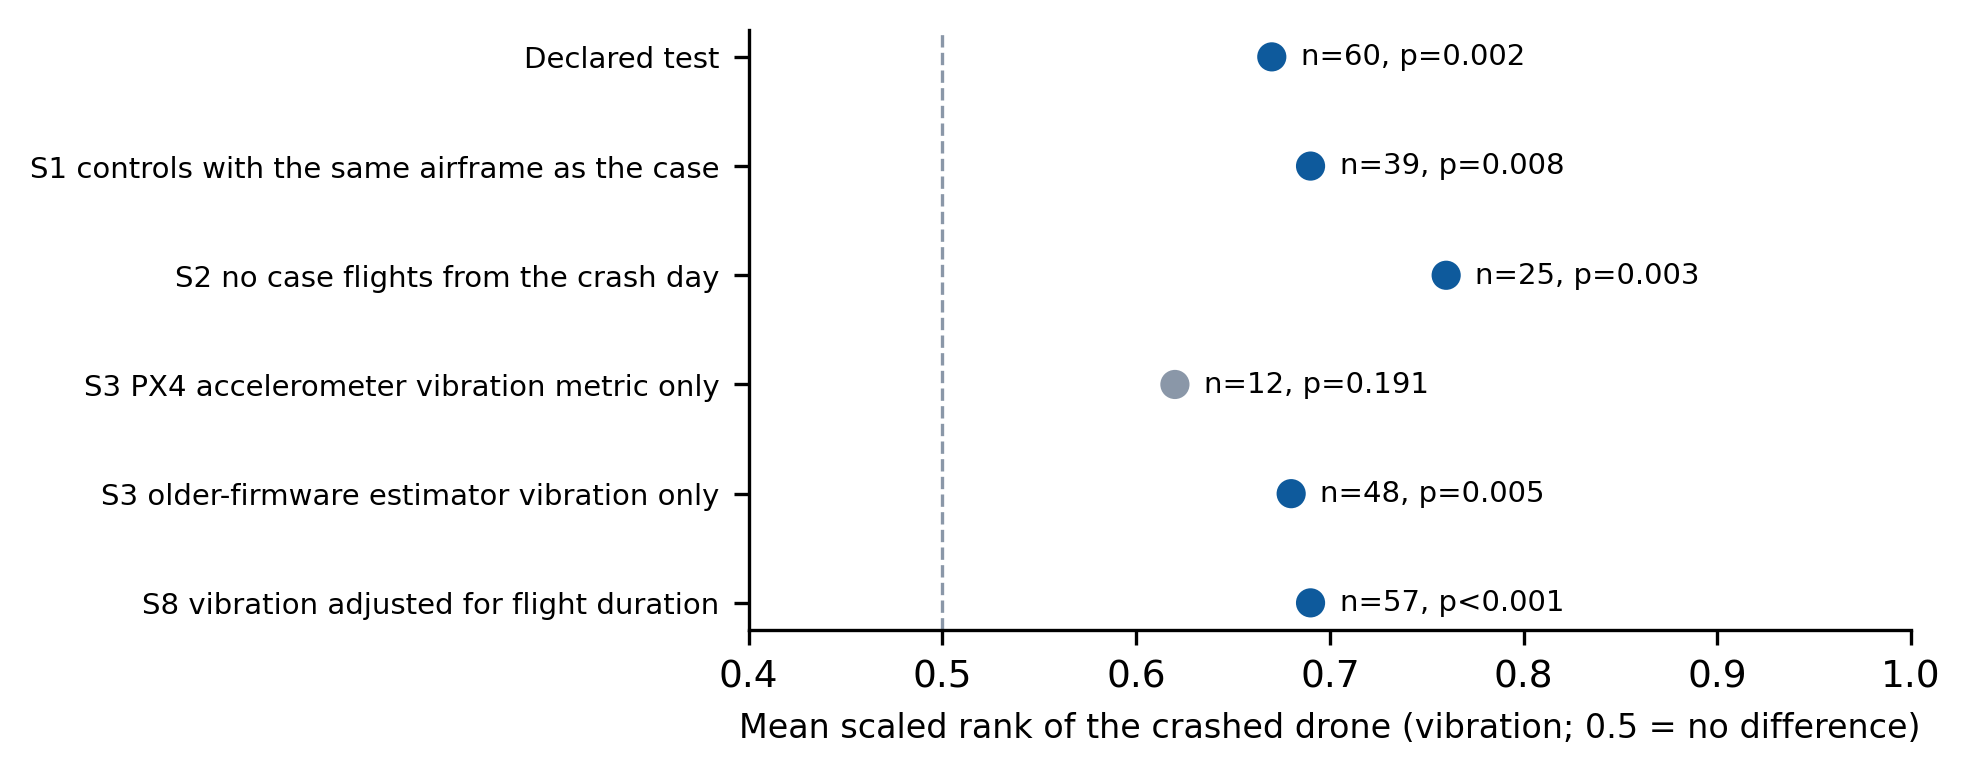
\includegraphics[width=0.78\textwidth]{fig_robustness.png}
\caption{Between-drone vibration result under alternative specifications (exploratory). Specification labels: S1: airframe-matched controls; S2: excluding case flights from the crash day; S3: stratification by vibration measurement source (older-firmware estimator metric vs.\ newer accelerometer metric); S8: log-linear adjustment for flight duration. Blue: $p<0.025$. These $p$-values treat sets as independent. $^\dagger$With one set per crashed airframe, median $p$ is 0.026 (S1), 0.023 (S2), 0.019 (older estimator metric), 0.28 (newer accelerometer metric), 0.019 and 0.014 (GPS-ordered variants); S8 was not re-run and remains unclustered.}
\label{fig:robust}
\end{figure}


\FloatBarrier

\section{Expert diagnoses: fault checks and attribution}
\label{sup:experts}
\paragraph{Check definitions} Fixed deterministic checks for
the five physical failure modes named by experts were evaluated:
(i)~\textit{Tuning}: combined roll and pitch rate-tracking RMS error $> 0.30$\,rad/s over at least 50 samples;
(ii)~\textit{Vibration}: total accelerometer clipping counts $> 50$ or 95th-percentile \texttt{accel\_vibration\_metric} $> 30$\,m/s$^2$;
(iii)~\textit{GPS/Compass}: \texttt{mag\_test\_ratio} $> 1.0$ in \texttt{estimator\_status} for $\ge 1.0$\,s cumulative, or horizontal position error $\text{eph} > 5$\,m or satellites $< 6$ for $\ge 5.0$\,s cumulative while in a GPS-dependent mode;
(iv)~\textit{Motor/ESC}: any motor output at $\ge 95\%$ authority (or PWM $\ge 1950$\,$\mu$s) for $\ge 1.0$\,s cumulative;
(v)~\textit{Battery}: battery warning level $\ge 2$ (critical/emergency) or state of charge $< 10\%$.
Checks were declared useful if they fired on at least 50\% of logs with that diagnosis and at most 10\% of normal flights,
evaluated first on the full window ($m=0$\,s) and then with the final 10\,s removed ($m=10$\,s).

Table~\ref{tab:checks} compares the fault checks with the full flight window ($m=0$\,s) and with the last 10\,s before
the crash removed ($m=10$\,s). With the window ending 10\,s before the crash, no check met the declared criterion.
The tuning check illustrates the diagnostic leakage described in Section~\ref{M-sec:window}: across all candidate logs with the full
window, the check fired on 10 of 12 (83.3\%). Across the 9 constant tuning logs with duration $\ge 10$\,s surviving the 10\,s
cut-off without sample attrition, firing dropped from 7 of 9 (77.8\%) with the full window to 1 of 9 (11.1\%) at $m=10$\,s
(6 logs lost firing, 0 gained; exact two-sided McNemar $p=0.03125$). However, normal-flight firing also fell from 18/142 (13\%)
to 7/130 (5\%), indicating that window shortening itself reduces cumulative exposure to threshold triggers alongside any crash-impact
leakage. The tuning check itself is defined as rate-tracking RMS above 0.30\,rad/s, a quantity that loss of control raises by definition, so its drop shows that this one rule-based check depends on the crash window rather than measuring a general leakage effect. $^\dagger$Its drop was also not clearly larger than the normal-flight drop: among flights that fired at the full window and could be scored at both cut-offs, crash logs lost firing in 6 of 7 and normal flights in 4 of 11 (one-sided Fisher exact $p=0.057$). Furthermore, this exploratory finding is descriptive rather than confirmatory: across the five diagnostic checks evaluated,
an unadjusted $p=0.031$ does not survive Bonferroni multiplicity correction ($p \approx 0.16$), and the other four checks exhibited
low baseline sensitivity even on full windows ($\le 25\%$, with 0/4 for motor and 0/2 for battery on paired logs), while tuning exceeded
the declared 10\% normal-flight false-alarm ceiling (13\%). Thus, while the rate-tracking check depended on the crash window, claims that
leakage is strictly confined to tuning must be tempered by the limited baseline sensitivity of the remaining checks.

To test diagnostic attribution on independently evaluated incidents, we evaluated the rule across all 43 downloadable logs behind
expert forum threads (38 aircraft-fault and 5 pilot-fault). As noted in Section~\ref{M-sec:data}, cross-tabulating these 43 logs against
archive ratings revealed that all 9 logs carrying an uploader rating were labeled \texttt{crash\_sw\_hw} (and all 9 were diagnosed as aircraft
faults by experts, 100\% agreement); the 5 expert pilot crashes were submitted unrated, which is consistent with, but not statistical
evidence of, reluctance to self-identify pilot fault: all 5 pilot logs were unrated in the index against 28 of 38 aircraft logs unrated
(one-sided Fisher exact $p=0.25$). Evaluated on the 38 aircraft incidents, the fixed rule predicted ``aircraft'' in 18 (47.4\%),
``unknown'' in 6 (15.8\%), and erroneously blamed the ``pilot'' in 14 (36.8\%). On decided aircraft cases ($n=32$), the rule was wrong on
43.8\% (14/32). Detailed inspection of flight mode sequences confirmed the failure mechanism: in all 14 misclassified logs, the vehicle was
in a pilot-flown mode at the crash moment (\texttt{POSCTL} in 7 logs, \texttt{STAB} in 4, \texttt{ALTCTL} in 3; including log \texttt{e9034973},
which transitioned \texttt{POSCTL} $\to$ \texttt{AUTO\_4} $\to$ \texttt{POSCTL} as the pilot attempted manual recovery). Because no hardware
failsafe fired before impact, the rule defaulted to blaming the pilot.

Conversely, when evaluated on the 5 pilot-fault incidents, the fixed rule predicted ``aircraft'' in 4 (80.0\%) and ``pilot'' in only 1 (20.0\%;
pilot recall 1 of 5, exact Clopper--Pearson 95\% CI 0.5--71.6\%, Wilson 3.6--62.4\%), misclassifying 4 of 5 pilot crashes because motor saturation,
accelerometer clipping, or failsafe activation occurred as the vehicle struck the ground. Combining both classes across all 37 decided expert logs
(32 aircraft, 5 pilot), the rule produced 18 incorrect decisions out of 37 (48.6\% error rate), yielding a balanced accuracy of
$(56.25\% + 20.0\%) / 2 = 38.1\%$ (Bayesian 95\% credible interval 0.25--0.61 from independent Jeffreys beta posteriors on the two recalls; exact 95\% intervals for the recalls themselves are 37.7--73.6\% for aircraft, 18 of 32, and 0.5--71.6\% for pilot, 1 of 5). The interval contains chance (0.50) and lies below 0.70, the pass mark declared for the rule on uploader labels (not for this expert set), so the rule probably falls below that mark here but cannot be separated from chance. When evaluated on the subset of 34 logs with complete telemetry required by the statistical models (30 aircraft, 4 pilot), the rule decided 29 cases (25 aircraft, 4 pilot), predicting aircraft in 15 of 25 aircraft and 4 of 4 pilot, yielding a balanced accuracy of $(60.0\% + 0.0\%) / 2 = 30.0\%$. Of the 30 complete aircraft logs, exactly 5 overlapped with the 148 modelled crashes in the training pool (all 5 rated \texttt{crash\_sw\_hw} in the index; 0 pilot logs overlapped). Evaluating the cross-validated logistic regression model across all 34 complete logs yielded predictions of ``aircraft'' in 27 of 30 aircraft logs (90.0\%) and in all 4 pilot logs (0/4 pilot recall; covering 4 of the 5 pilot logs because one lacked actuator or setpoint topics), defaulting strongly toward its aircraft training prior (75.7\% prevalence; 112/148) for a balanced accuracy of $(90.0\% + 0.0\%) / 2 = 45.0\%$ and ROC AUC of $0.467$ (95\% bootstrap CI 0.211--0.733). When the 5 overlapping logs were excluded ($n=29$: 25 aircraft, 4 pilot), the logistic regression model achieved AUC 0.450 (95\% bootstrap CI 0.185--0.715); given the wide confidence interval spanning from 0.185 to 0.715 on 29 logs, this evaluation provides no evidence of discrimination and remains inconclusive. Across both heuristic rules and statistical models on this sample, log-based telemetry attribution showed no discriminative agreement above chance. We emphasize the caveat
that this evaluation measures agreement between heuristic rules or models and expert community reading of the same telemetry, rather than ground truth:
original posters explicitly confirmed the diagnosis in only 47 of 94 aircraft-fault threads (50.0\%) and 5 of 9 pilot-fault threads (55.6\%).
Nonetheless, this independent evaluation illustrates the challenge of log-based attribution: neither the heuristic rule nor the statistical model demonstrated reliable agreement above chance.

\begin{table}[t]
\centering
\caption{Fault checks on logs whose expert named the matching fault, with the full window ($m=0$\,s) and with the last 10\,s
before the crash removed ($m=10$\,s). Declared criterion: at least 50\% of diagnosed logs and at most 10\% of normal flights.
Paired columns show constant logs surviving across both windows.}
\label{tab:checks}
\footnotesize
\setlength{\tabcolsep}{2.5pt}
\begin{tabularx}{\textwidth}{@{}Xcccccc@{}}
\toprule
 & \multicolumn{2}{c}{Diagnosed ($m=0$\,s)} & Diagnosed & Paired $\Delta$ & \multicolumn{2}{c}{Normal comparison} \\
\cmidrule(lr){2-3} \cmidrule(lr){4-4} \cmidrule(lr){5-5} \cmidrule(lr){6-7}
Expert-named fault & All logs & Paired & $m=10$\,s & ($p$-value) & $m=0$\,s & $m=10$\,s \\
\midrule
Tuning or configuration & 10/12 (83\%) & 7/9 (78\%) & 1/9 (11\%) & $-6$ ($p=0.031$) & 18/142 (13\%) & 7/130 (5\%) \\
Vibration or mounting & 3/5 (60\%) & 3/5 (60\%) & 3/5 (60\%) & 0 ($p=1.00$) & 7/48 (15\%) & 4/38 (11\%) \\
GPS, compass or estimator & 1/5 (20\%) & 1/4 (25\%) & 1/4 (25\%) & 0 ($p=1.00$) & 10/143 (7\%) & 5/130 (4\%) \\
Motor, ESC or propeller & 1/9 (11\%) & 0/4 & 0/4 & 0 ($p=1.00$) & 8/143 (6\%) & 5/130 (4\%) \\
Battery or power & 0/4 & 0/2 & 0/2 & 0 ($p=1.00$) & 4/143 (3\%) & 1/130 (1\%) \\
\bottomrule
\end{tabularx}
\end{table}

\begin{figure}[t]
\centering
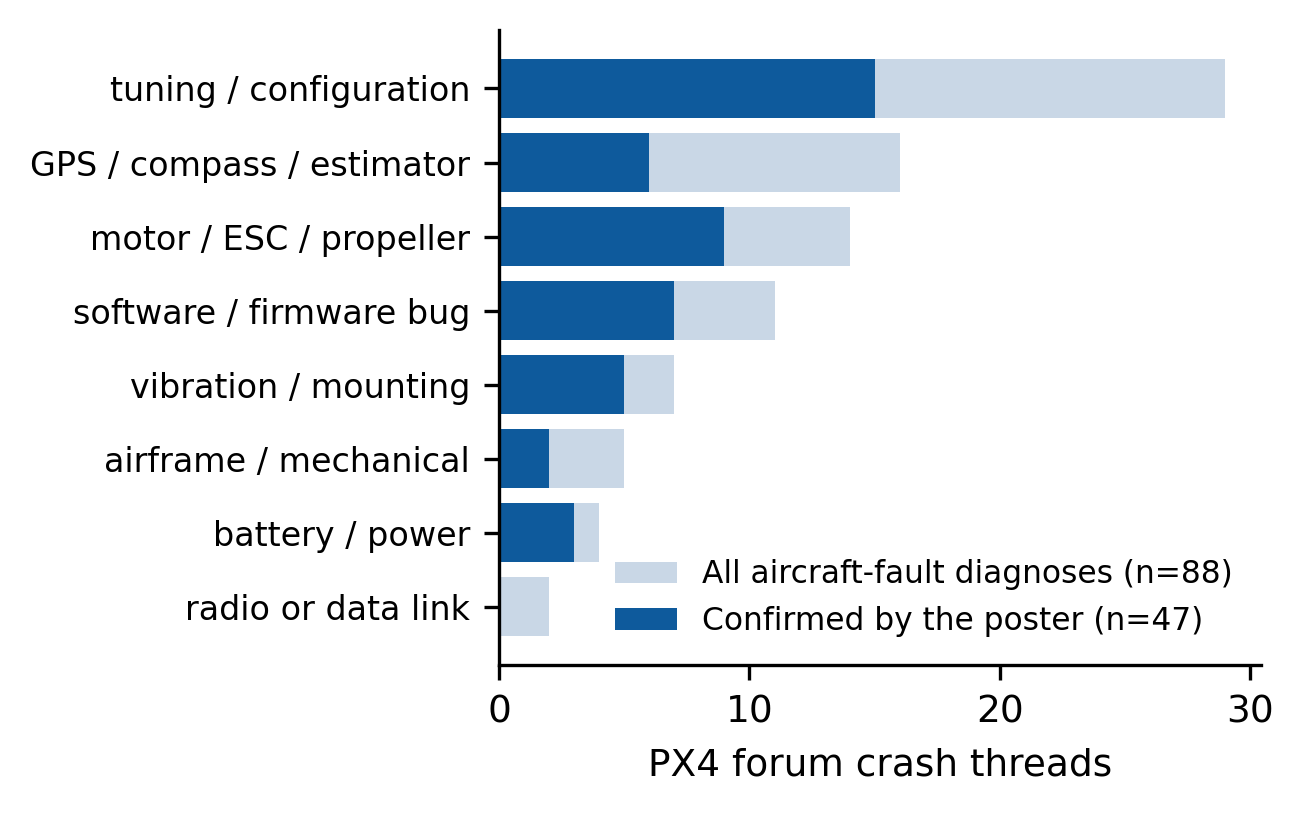
\includegraphics[width=0.78\textwidth]{fig_forum_causes.png}
\caption{Causes named by experts in PX4 forum threads that attributed a crash to the aircraft.}
\label{fig:causes}
\end{figure}


\FloatBarrier

\section{A published log checker (FlightMD): details}
\label{sup:flightmd}
$^\dagger$To see whether these patterns are particular to our features and models, we re-evaluated an independent tool. FlightMD \cite{flightmd2026} is an open-source, rule-based PX4 log checker whose author validated it on 50 Flight Review logs; it is not peer-reviewed. Seven scored modules (oscillation, vibration, estimator, battery, GPS, parameters, motors) raise findings that the tool combines into a 0--100 health score; its eighth check, an ascent and recovery profile for rockets and balloons, is outside the score and was not run. We ran its parser, analysers and score calculator unchanged (commit \texttt{306d0cb}), but not its full pipeline, which sends the log's GPS position to external weather and place-name services and has an optional language-model step that does not affect the score. The protocol, samples and wording rules were declared before any study log was scored (\texttt{fa5fb0b}); logs were cut at the crash moment as in Section~\ref{M-sec:crashwindow}. Because the tool is not trained, fold grouping does not apply; intervals come from a vehicle-cluster bootstrap.

On the constant cohort (89 crashes, 124 normal flights) the health score separated crashes from normal flights with AUC 0.79 [0.67, 0.87] on the whole log, 0.74 [0.61, 0.83] up to the crash moment and 0.72 [0.58, 0.81] with the last 10\,s removed, so it separates crash flights from other drones' flights before the crash window. Post-crash data and the last 10\,s raised AUC by 0.048 [0.018, 0.089] and 0.025 [0.002, 0.054], both below the declared 0.05 rule (on the 24 tilt-defined multicopter crashes, 0.066 and 0.037). Most of the separation came from the estimator module (mean module score 63 in crashes against 92 in normal flights at $m=10$\,s). Against the drone's own earlier flights the same score gave no warning (crash-flight rank 0.48, $p=0.66$, 46 drones). Taking ``any critical finding'' as an aircraft verdict, it reached a balanced accuracy of 0.52 [0.44, 0.61] against the uploader labels at the crash moment and 0.48 [0.38, 0.59] with the last 10\,s removed, below the 0.70 pass mark; its score did not separate the labels either (AUC 0.47 [0.37, 0.57]). It rated 1.4\% of normal flights below 60 (``Warning'' or worse) but also only 9\% of crashes. An independent tool therefore shows the same pattern as our own pipeline: separation between aircraft, no warning within an aircraft, and no attribution.
\FloatBarrier

\section{Injected-fault control: details}
\label{sup:rflymad}
$^\dagger$The archive cannot separate a tool that fails from labels that fail. RflyMAD \cite{le2025rflymad} can: its real flights carry faults injected in the PX4 firmware (motor efficiency loss and sensor faults on three multicopters, one operator), and each log records the injection in a dedicated topic, so the cause and its onset time are known. We downloaded the real-flight subset from its Kaggle copy and declared the analysis before scoring any log (\texttt{a9877c1}). Of 493 logs, 5 in fault folders had no fault code and were excluded, leaving 240 motor-fault, 197 sensor-fault and 51 fault-free flights (the Kaggle copy has 51 fault-free real flights, not the 84 the dataset page lists, and 245 motor-fault logs, of which 240 carry a fault code, against the 231 real motor-fault flights the page lists). Onset came from the log, not from the per-case workbooks, one of which described a different case. Fault-free flights were given a pseudo-onset at the median onset time of fault flights with the same flight pattern. Windows ran from take-off to the onset (``pre''), to 10\,s after it, and to the end of the flight.

The declared attribution rule, unchanged, called 8 of 240 motor-fault flights (3\%) and 10 of 197 sensor-fault flights (5\%) aircraft-caused, against 2 of 51 fault-free flights (4\%); its balanced accuracy for motor faults against fault-free flights was 0.50 [0.47, 0.52], below the 0.70 that would have shown it recognises known aircraft faults. Its signs are built for crashes (saturated motors, clipping, failsafes, warnings) and did not fire on a 15--20\% loss of motor efficiency that the controller absorbed. FlightMD's health score did not separate faulty from fault-free flights before the fault (AUC 0.47 [0.39, 0.55]) or with 10\,s of it (0.51 [0.44, 0.58]), but did on the whole flight (0.69 [0.63, 0.75]).

The study's 11 features did the opposite. A logistic model separated faulty from fault-free flights at AUC 0.86 (permutation $p=0.005$) using only data from \emph{before} the fault was injected; including 10\,s of the fault changed this by $-0.008$ [$-0.033$, 0.018], and the whole flight gave 0.82. The separation held within each flight pattern (pooled 0.88) and, in a check we had not declared, on the four days when both classes were flown (0.82, 163 flights). It came mainly from tilt and rate-tracking error (single-feature AUC 0.86 and 0.81): the fault flights were flown more aggressively before the injection. A fault-versus-normal classifier on this dataset can therefore score well with no fault present, which is the between-flight confounding of Section~\ref{M-sec:factorial} in a setting where the cause is known. Both results bound the archive findings: the rule's failure there partly reflects signs that miss faults the controller absorbs, not only noisy labels; and a high crash-versus-normal AUC is weak evidence of a fault signal unless a pre-onset or same-flight baseline is reported.

\paragraph{Folds grouped by day and by flight pattern (declared \texttt{e45b583})} The stratified folds above can let a model recognise a session. Grouping folds by flight date (18 days, only 4 of which include fault-free flights) gave AUC 0.747 before the fault, 0.710 with 10\,s of it and 0.538 for the whole flight (permutation $p=0.005$, 0.005 and 0.16); fault minus pre-fault $-0.038$ [$-0.080$, 0.005]. Grouping by flight pattern (5 patterns) gave 0.789, 0.771 and 0.699 (all $p=0.005$); fault minus pre-fault $-0.017$ [$-0.048$, 0.013]. By the declared rule the pre-fault separation ``survives grouping by day''.

\paragraph{Within the four mixed days and window lengths (declared \texttt{1e0bf0f})} Only 4 of the 18 days contain fault-free flights, so a leave-day-out AUC pools test folds that contain one class only. Within each of the four mixed days (16, 61, 41 and 45 flights; 11, 10, 20 and 10 fault-free), the day-grouped out-of-fold scores gave pre-fault AUC 0.964, 0.851, 0.317 and 0.683 (size-weighted mean 0.681), fault-window AUC 0.945, 0.798, 0.557 and 0.763 (0.742) and whole-flight AUC 0.364, 0.643, 0.781 and 0.631 (0.647). The pooled day-grouped whole-flight AUC (0.538, $p=0.16$) is lower than the stratified 0.82 because whole flights differ in length and content far more across days than within them. Median pre-fault windows were 36\,s for fault flights and 20\,s for fault-free flights (the pseudo-onset), and median whole flights 111\,s and 69\,s; 47\% and 39\% of whole flights exceeded 120\,s. Permutation $p$-values reported as 0.005 are the smallest possible with 200 permutations ($p\le0.005$).

\paragraph{Window length (declared \texttt{031fdd6})} Window length alone separates fault from fault-free flights at AUC 0.667 (pre-fault window) and 0.599 (whole flight). With every flight's pre-fault window cut to the same span after take-off (the pseudo-onset offset of its flight pattern, or the injection if earlier), the study's features gave AUC 0.856 with stratified folds and 0.749 with folds grouped by day (both $p\le0.005$, 200 permutations), essentially unchanged; by the declared rule the separation survives length matching.
\FloatBarrier

\section{Language-model review panels}
\label{sup:lm}
\paragraph{Panel design} The panel tested a design proposed for advisory diagnosis: several reviewers, each
restricted to one slice of evidence (navigation, pilot inputs, GPS, battery, settings), vote on a fixed list of six
causes and must cite numbered facts extracted from the log. Robustness was evaluated by replacing one reviewer with an
adversary arguing for a chosen wrong cause, and planting hostile strings in uploader-controlled fields. 

\paragraph{Real-log cases and label mapping (declared \texttt{5b15715}, amended \texttt{7405264})} The 97 real cases are 35 forum crashes, labelled with the forum experts' cause, and 62 crashes from the blind relabelling, labelled with the reviewer's main cause (the reviewer's pilot, aircraft and environment verdict is not used directly; cases the reviewer marked ``can't tell'' are excluded). Causes were mapped to the panel's list before any run: pilot input or handling, wrong mode or mode switch, and flew into an obstacle or the ground $\to$ pilot manual control; GPS, compass or estimator $\to$ GPS degraded; wind or environment $\to$ wind or environment; battery or power $\to$ low battery response; tuning or configuration $\to$ configuration. Every other cause (motor, ESC or propeller; vibration; software; airframe; radio; not stated; no crash visible; not enough data) has no place in the panel's list, so the right answer for those 21 cases is to defer to a person. Facts were extracted from the last 20\,s of each log by the tool's own parser and fact builder; no author wrote a case. Because 62 of the labels come from one reviewer working from plots, a ``wrong'' answer means disagreement with a contested label, not a demonstrated error.

\subsection*{Exploratory evaluation of language-model review panels (preliminary)}

Because language-model assistants are increasingly proposed for automated flight log analysis, we conducted a preliminary exploratory evaluation on 60 author-generated fault cases using four local models (3--4B parameters) configured both as single agents and as multi-agent review panels (Table~\ref{tab:llm}). While a fixed deterministic rule achieved 75\% accuracy (naming the true cause in 35 of 50 active cases and correctly abstaining on 10 no-cause cases) with 0\% error (referring 15 cases to human operators), local language models produced substantial error rates (10--63\% wrong), suffered from mode collapse or complete abstention on active causes, and proved highly vulnerable to consensus manipulation: in a worst-case sensitivity sweep, a single compromised reviewer systematically flipped the panel's consensus decision in 45 to 56 of the 60 cases. In contrast, deterministic numeric telemetry extraction into code prevented direct prompt injection by construction across 40 hostile input strings. This exploratory comparison indicates that the tested small local models and review-panel configurations were unreliable on the 60 author-generated cases. Because the cases and fixed rule were developed by the same authors, the comparison is not an independent benchmark and should not be generalized to language models as a class or larger architectures. These preliminary results emphasize that multi-agent consensus voting without cryptographic proofs or fact-citation constraints cannot provide dependable safety assurance.

$^\dagger$\emph{Blind real-log cases.} To remove the authors from the cases, we repeated the comparison on 97 real crash logs (declared \texttt{5b15715}, amended \texttt{7405264}): 35 from forum threads with expert-diagnosed causes and 62 from the independent relabelling (Section~\ref{M-sec:attribution}). No case was written by an author: the tool's own parser and fact builder extracted each case's facts from the last 20\,s of the log, and the labels were mapped to the panel's causes before any run; 21 cases had a cause outside the panel's list (motor, vibration, software and similar), where the right answer is to defer. The four models were run on an NVIDIA RTX~4060 laptop with the same model versions (the runner's note lists the declared model IDs; the models were removed before \texttt{ollama list} was captured). The rule's answers and the labels matched a local recomputation on all 388 rows. Table~\ref{tab:llm_real} gives the results. The fixed rule, which looked flawless on the generated cases, named a wrong cause in 62 of 97 real crashes (64\%) and was right in 26. By the declared criterion (more right answers and no more wrong ones than the rule) no panel beat it, so the conclusion that such panels are not recommended stands. Single agents gemma3 and phi4-mini were never wrong, but only because they deferred about three quarters of the cases; with a single compromised reviewer the panel switched to the attacker's cause in 83 to 89 of 97 cases (16 for qwen2.5). On the 33 cases also run on the authors' Mac, the rule and the single agent gave identical answers on both machines, but the five-reviewer panel did so in only 16, so at temperature~0 the panel's verdict still depended on the hardware. On real logs, then, neither the rule nor any model named the cause reliably: the generated cases had flattered the rule.

\begin{table}[!htbp]
\centering
\caption{$^\dagger$Rule and language models on 97 real crash logs with independent labels (35 forum-expert, 62 blind relabelling; 21 with a cause outside the panel's list, where deferring is right): right (R), wrong (W) and deferred (Def) counts. Flips: cases in which one compromised reviewer moved the panel to its target cause.}
\label{tab:llm_real}
\footnotesize
\begin{tabular*}{\textwidth}{@{\extracolsep{\fill}}l ccc@{}}
\toprule
Method & Single agent R / W / Def & Review panel R / W / Def & Flips / 97 \\
\midrule
Fixed rule (no model) & 26 / 62 / 9 & -- & -- \\
\texttt{gemma3:4b} & 21 / 0 / 76 & 12 / 57 / 28 & 83 \\
\texttt{phi4-mini} & 23 / 0 / 74 & 17 / 40 / 40 & 89 \\
\texttt{qwen2.5:3b} & 27 / 70 / 0 & 26 / 69 / 2 & 16 \\
\texttt{qwen3:4b} & 23 / 28 / 46 & 20 / 35 / 42 & 88 \\
\bottomrule
\end{tabular*}
\end{table}

\begin{table}[!htbp]
\centering
\caption{Language-model review panels on 60 generated cases: counts of right (R), wrong (W), and deferred (Def) cases, with coverage (Cov., share of cases decided) and accuracy when answering (Acc.). ``Right'' includes correctly leaving a no-cause case open. Single-agent gemma3 and phi4 answered only the 10 no-cause cases (0\% coverage on active causes). Adversary flips show consensus changes caused by a single compromised reviewer in a worst-case sweep.}
\label{tab:llm}
\footnotesize
\setlength{\tabcolsep}{2.5pt}
\begin{tabular*}{\textwidth}{@{\extracolsep{\fill}}l ccc ccc c@{}}
\toprule
& \multicolumn{3}{c}{Single agent} & \multicolumn{3}{c}{Review panel} & Compromised \\
\cmidrule(lr){2-4} \cmidrule(lr){5-7}
Method & R / W / Def & Cov. & Acc. & R / W / Def & Cov. & Acc. & Flips / 60 \\
\midrule
Fixed rule (no model) & 45 / 0 / 15 & 75\% & 100\% & -- & -- & -- & -- \\
\texttt{gemma3:4b} & 10 / 0 / 50 & 17\%$^{a}$ & 100\%$^{a}$ & 3 / 36 / 21 & 65\% & 7.7\% & 49 \\
\texttt{phi4-mini} & 10 / 0 / 50 & 17\%$^{a}$ & 100\%$^{a}$ & 20 / 19 / 21 & 65\% & 51.3\% & 56 \\
\texttt{qwen2.5:3b} & 9 / 44 / 7 & 88\% & 17.0\% & 10 / 6 / 44 & 27\% & 62.5\% & 54 \\
\texttt{qwen3:4b} & 0 / 41 / 19 & 68\% & 0.0\% & 17 / 38 / 5 & 92\% & 30.9\% & 45 \\
\bottomrule
\end{tabular*}
\vspace{2pt}
{\footnotesize $^{a}$Answered only on the 10 no-cause cases where abstention coincided with the ground truth; 0\% coverage on active causes.\par}
\end{table}


\FloatBarrier

\section{A published trained detector: re-implementation and results}
\label{sup:trained}
\paragraph{The detector} The RflyMAD authors report fault diagnosis with an improved LeNet-5 convolutional network on 12 flight signals (velocity, angular velocity, acceleration and Euler angles, three axes each), trained for 10 epochs, with 98.2\% accuracy on real single-motor faults in hover (simulation plus 10\% real data) and 89.7--99.1\% across settings \cite{le2025rflymad}. Their description gives neither code, weights, window length, sampling rate nor split. Our re-implementation (declared \texttt{1e0bf0f} before any training) uses: \texttt{vehicle\_local\_position} $v_x, v_y, v_z$, \texttt{vehicle\_angular\_velocity}, \texttt{vehicle\_acceleration} and roll, pitch and yaw from \texttt{vehicle\_attitude}, linearly resampled to 10\,Hz over the airborne armed period; non-overlapping 32-sample (3.2\,s) windows; per-channel standardisation fitted on the training fold; a one-dimensional LeNet-5 over time (Conv 12$\to$6, kernel 5, batch normalisation, ReLU, max-pool 2; Conv 6$\to$16, kernel 5, batch normalisation, ReLU, max-pool 2; fully connected 80$\to$120$\to$84$\to$2); Adam, learning rate $10^{-3}$, batch 64, 10 epochs.
\paragraph{Data} 240 motor-fault and 51 fault-free RflyMAD real flights (291 flights). A window is a fault window if it lies wholly between injection and the end of the fault (2,258 windows), a pre-fault window if it lies wholly before the injection (3,013); fault-free flights give 1,548 normal windows, 506 of them before the pseudo-onset.
\paragraph{Results} Fault versus normal windows: random 80/20 window split, accuracy 0.878 and AUC 0.943 (mean of five seeds); five-fold cross-validation grouped by flight, 0.858 and 0.921; grouped by flight day, 0.621 and 0.626. A window-level cross-validation over all windows gave AUC 0.964 against 0.635 for day grouping, a difference of 0.329 [0.276, 0.381] (flight-level bootstrap). Pre-fault windows of fault flights against normal windows before the pseudo-onset, where no fault exists in either class: AUC 0.849 grouped by flight and 0.567 grouped by day. All grouped conditions had flight-level permutation $p\le0.0099$ (100 permutations, null means 0.48--0.49). Accuracy for the pre-fault task is not informative because 86\% of its windows are positive. By the declared rules the published accuracy was not reproduced on a random split (0.878 $<$ 0.90), the random split inflates the detector (difference $\ge 0.05$ with an interval excluding zero), and the detector separates fault flights with no fault present (AUC $\ge 0.70$, $p<0.05$).
\paragraph{By day and with matched windows (declared \texttt{031fdd6}, amended \texttt{72efcac})} Of the four days with fault-free flights, one (15 June 2023) has no motor-fault flights, so it has no AUC; the amendment takes the mean over the other three. Day-held-out detector scores within each day: fault versus normal 0.828, 0.643 and 0.340 (size-weighted mean 0.603); pre-fault 0.765, 0.478 and 0.380 (0.505). With pre-fault windows limited, for every flight, to the span after take-off that fault-free flights use (3,241 windows): AUC 0.847 with flights held out (flight-level permutation $p=0.0099$) and 0.533 with days held out ($p=0.12$). By the declared rule the detector ``separates fault flights before the fault even with matched windows'' when flights are held out; it does not when days are held out.

\paragraph{Limits} This is a re-implementation from a description, not the authors' model; it was trained on real flights only, without the simulation data the authors used, and on three airframes flown by one team. The fault-free flights come from 4 of 18 days, so day-grouped folds include folds with one class only.
\FloatBarrier

\section{Revision log: analyses added after the declared protocol}
\label{sec:posthoc}

\label{sec:posthoc}
To preserve the boundary between pre-declared confirmatory hypotheses (committed to version control on 20--24 October 2026; Table~\ref{M-tab:registration}) and exploratory analyses added after the declared protocol \cite{nosek2018prereg}, Table~\ref{tab:posthoc} documents each such analysis, its motivation, key results, git commit hash, first archive date in Software Heritage, and analysis run date. They are marked with $^\dagger$ throughout the text and tables. None of these exploratory additions altered the conclusions of the pre-declared tests. They bounded between-airframe confounding, tested other model types, quantified fleet screening, and audited the crash records themselves: the crash moment, the uploader labels against log content, and the order of flights.

{\scriptsize\setlength{\tabcolsep}{2.5pt}
\begin{longtable}{@{}p{0.19\textwidth}p{0.17\textwidth}p{0.42\textwidth}p{0.09\textwidth}p{0.09\textwidth}@{}}
\caption{Exploratory analyses added after the declared protocol, their motivation, key results, git commit hashes, the four commits archived in Software Heritage on 25 October 2026 (\nolinkurl{swh:1:rev:bad06ff1256865c7e63d44389aac174e0281291d}, \nolinkurl{swh:1:rev:bbdd0420de4547ac7d67b84165292a46237b604d}, \nolinkurl{swh:1:rev:624dd694e0d207dd9c44b1c9550faaf04453bc56}, and \nolinkurl{swh:1:rev:3a9aa89417fa9ea2a2334e3a4794e2358fb713ee}), and analysis run dates. Later commits are not yet archived.}\label{tab:posthoc}\\
\toprule
Analysis & Motivation & Key result & Commit & Run \\
\midrule
\endfirsthead
\toprule
Analysis & Motivation & Key result & Commit & Run \\
\midrule
\endhead
1,000-permutation null (Task B)$^\dagger$ & Calibrate detection threshold & Null mean 0.497; observed AUC upper bounds 0.510--0.619 (80\% power MDE 0.75); superseded by the refit permutation null (upper bounds $\le 0.69$, MDE 0.72) & \texttt{bad06ff} & 2026-10-25 \\
Depth-1 decision stumps (Task B)$^\dagger$ & Test single-feature non-linear splits & Stumps AUC $0.430 \to 0.413$ at $m=10$\,s (upper bounds 0.534 and 0.528); superseded by the refit null (0.447 and 0.481) & \texttt{bad06ff} & 2026-10-25 \\
Constant-subset leak curve$^\dagger$ & Exclude sample attrition ($n=213$) & AUC declines smoothly $0.895 \to 0.868$ ($m=10$\,s) & \texttt{bbdd042} & 2026-10-25 \\
Paired diagnostic leakage test$^\dagger$ & Test leakage on constant logs ($n=9$) & Tuning check $7/9 \to 1/9$, exact McNemar $p=0.03125$ & \texttt{bbdd042} & 2026-10-25 \\
Same-sample decomposition$^\dagger$ & Account for airframe \& duration confounds & Changing comparison from other aircraft to same aircraft lowers AUC 0.83--0.88 to 0.53--0.57; superseded by the factorial audit, in which fold grouping was the only material factor & \texttt{eb463b5} & 2026-10-25 \\
Poisson-binomial set null$^\dagger$ & Account for mixed set sizes ($n=60$) & Exact null rate 40.28\%; observed 55.0\% ($p=0.0137$) & \texttt{bad06ff} & 2026-10-25 \\
Screening PPV and CIs$^\dagger$ & Quantify operational fleet value & Exploratory illustration: fleet PPV 2.26--2.43\% (exact Bayes) at assumed 10\% flag rate ($3.3\times$ lift); withdrawn, superseded by the measured reference below & \texttt{bad06ff} & 2026-10-25 \\
Sensitivity by vibration source$^\dagger$ & Compare older vs.\ newer metrics & Older: 32/48 (66.7\%); newer: 6/12 (50.0\%); pooled newer $\bar r=0.58$ ($p=0.25$) & \texttt{624dd69} & 2026-10-25 \\
Independent 43-log validation$^\dagger$ & Evaluate against independent causes & Balanced accuracy 0.381 (95\% CrI 0.25--0.61); pilot recall 1/5; inconclusive & \texttt{3a9aa89} & 2026-10-25 \\
Cohort selection step 4b$^\dagger$ & Isolate comparison vs.\ cohort effect & 67 multi-flight crashes vs.\ other-aircraft controls: AUC 0.522 [0.413, 0.615]; superseded by the factorial audit (mixed extractors) & \texttt{f152d07} & 2026-10-26 \\
Within-drone duration caliper$^\dagger$ & Test duration confounding in cohort & Caliper $\le 0.25$ matching lifts within-drone AUC $+0.110$ (0.532 to 0.642) & \texttt{f152d07} & 2026-10-26 \\
Depth-3 tree bounds across cuts$^\dagger$ & Bound non-linear model performance & Upper bounds 0.519--0.724; superseded by the refit permutation null (0.54--0.69) & \texttt{dfbabaf} & 2026-10-26 \\
Fixed-score permutation null$^\dagger$ & Test CV fold-splitting variance & Fixed score SD 0.055 matches asymptotic theory (0.056); 0.090 reflects refitting variance & \texttt{dfbabaf} & 2026-10-26 \\
Control cluster adjustment$^\dagger$ & Test control reuse robustness & Mean rank 0.665, 95\% cluster CI [0.587, 0.744]; heterogeneity $p=0.322$ & \texttt{dfbabaf} & 2026-10-26 \\
Single vs.\ multi-history crashes$^\dagger$ & Test maiden-flight artifact hypothesis & Single-history ($n=45$) AUC 0.835 vs.\ multi-history ($n=103$) 0.891 at $m=0$\,s; cross-sectional separation is archive-wide & \texttt{aa1d7c6} & 2026-10-26 \\
Duration caliper gradient \& CI$^\dagger$ & Quantify caliper sensitivity & Lift curve $\epsilon \in [0.10, 1.00]$; paired cluster bootstrap 95\% CI for $\Delta=+0.125$ is [+0.074, +0.238]; superseded by the reproducible rerun [+0.028, +0.205] & \texttt{aa1d7c6} & 2026-10-26 \\
Two-stage cluster bootstrap \& GPS$^\dagger$ & Audit same-day timing \& clustering & Two-stage cluster CI [0.536, 0.789] (resampled drones counted once; corrected to [0.50, 0.81]); same-day check compared dates only; superseded by the GPS flight-order audit & \texttt{aa1d7c6} & 2026-10-26 \\
Rule balanced accuracy across cuts$^\dagger$ & Audit attribution rule across margins & Feature-based proxy of the rule: BA 0.46 [0.38, 0.54] ($m=0$\,s) to 0.45, 0.39, 0.37, 0.35 [0.25, 0.45] ($m=30$); below 0.5 from low pilot recall, not undecided cases & \texttt{aa1d7c6} & 2026-10-26 \\
Archive-wide label audit$^\dagger$ & All 520 crash-rated logs & 39\% of 341 readable multicopter logs show a tilt event; share containing the crash 50--86\% depending on reviewer; pilot-rated 23\% vs aircraft-rated 45\% ($p=0.0003$) & \texttt{09cf99c}, \texttt{18b0eff} & 2026-10-27 \\
Label, detector and tilt-defined audit$^\dagger$ & Era-adjusted label link; objective crash detector; window analyses on tilt-defined crashes & Adjusted OR 2.08 [1.17, 3.69]; detector failed gate ($\kappa$ 0.72 and 0.38; 64\% false alarms); tilt-defined window effect 0.067 [0.015, 0.131] & \texttt{35103da} & 2026-10-28 \\
Aircraft-type and label-link audit$^\dagger$ & Tilt rule applied to mixed aircraft types; could the window effect be mechanical; is tilt a proxy for the label; a multi-cue crash detector & Multicopter tilt-defined effect 0.089 [0.019, 0.168], 0.131 [0.042, 0.226] without tilt/stick; all 15 reviewed multicopter tilt moments correct for both reviewers; tilt-alone AUC 0.53; within-stratum attribution 0.63 ($p=0.10$) and 0.62 ($p=0.11$); rule proxy BA 0.46 [0.38, 0.54]; multi-cue detector failed gate ($\kappa$ 0.82 and 0.32; 32\% false alarms) & \texttt{9650a69} & 2026-10-29 \\
FlightMD re-evaluation$^\dagger$ & Test a published open-source log checker under this protocol & Crash vs normal AUC 0.79 whole log, 0.74 at $t_c$, 0.72 [0.58, 0.81] at $m=10$\,s; window drops below 0.05; attribution BA 0.52 [0.44, 0.61]; within-drone rank 0.48 ($p=0.66$); 1.4\% of normal flights below 60 & \texttt{fa5fb0b} & 2026-10-29 \\
RflyMAD injected faults$^\dagger$ & Known-cause positive control on 488 real flights & Rule BA 0.50 [0.47, 0.52] (3\% of motor faults called aircraft); FlightMD 0.47 pre-fault, 0.69 whole flight; features AUC 0.86 pre-fault ($p=0.005$), fault adds $-0.008$; within flight pattern 0.88 & \texttt{a9877c1} & 2026-10-29 \\
Third rater$^\dagger$ & Non-author rater on the blind crash-moment sheet & Moment right: Fleiss' $\kappa$ 0.71 [0.53, 0.86]; contains crash: 0.33 [0.05, 0.58]; sided with blind reviewer on 11 of 13 disputed logs; majority archive estimate 80\% [68, 92] & \texttt{fdb3b7c} & 2026-11-01 \\
Independent relabelling$^\dagger$ & Blind non-author relabelling of 72 crashes from plots & Agreement with uploader $\kappa=-0.10$ [$-0.34$, 0.17]; 16/36 pilot-rated called aircraft; rule vs.\ reviewer BA 0.55 [0.42, 0.66]; FlightMD 0.52; tilt AUC 0.54 & \texttt{fa5fb0b} & 2026-11-01 \\
Operator clustering$^\dagger$ & Cluster the between-drone test by operator (location proxy, 2\,km) & 40 crashed airframes from 23 sites; site-clustered $p=0.006$ (Holm 0.042); one set per site median $p=0.14$; kept as suggestive (deviation from declared rule) & \texttt{cfb79b9} & 2026-11-01 \\
Screening reference$^\dagger$ & Rebuild reference from 412 non-crash drones; measure flag rates & Nominal 10\% flagged 13.7\%; lift $1.77\times$ [1.00, 2.60]; AUC 0.65; not shown to beat random inspection & \texttt{4961234} & 2026-11-01 \\
Blind real-log panel test$^\dagger$ & Rule and four local models on 97 real crash logs with independent labels & Rule 26 right / 62 wrong; no panel beats it; single agents defer $\sim$77\%; flips 16--89; Mac vs RTX panel agreement 16/33 & \texttt{5b15715}, \texttt{7405264} & 2026-11-02 \\
Dependence and control checks$^\dagger$ & Grouped folds for the injected-fault control; attribution on multicopters; site-weighted between-drone test; screening flag rates; touchdown pseudo moment & Pre-fault AUC 0.75 (by day); multicopter rule 0.43, models near chance after Holm; site-weighted $p=0.076$ (suggestive); leave-one-out lift $1.68\times$ [0.94, 3.31]; leak drops unchanged & \texttt{e45b583} & 2026-11-02 \\
Published trained detector and control details$^\dagger$ & Re-implement the RflyMAD LeNet-5 detector and test it under this protocol; per-day injected-fault AUC; third rater by type; rule on decided multicopter crashes & Detector AUC 0.94 (random windows) to 0.63 (days held out); 0.85 before the fault; per-day pre-fault AUC 0.32--0.96; third rater 13/15; decided multicopter BA 0.46 & \texttt{1e0bf0f} & 2026-11-03 \\
Crash-moment share, detector by day, length checks$^\dagger$ & Recompute the share of crashes the tilt rule misses on multicopters; detector per day and with matched windows; window-length AUC and length-matched features & Missed 7--50\% by rater; detector per-day pre-fault mean 0.51, matched 0.85 (flights) and 0.53 (days); length AUC 0.67; matched features 0.75 by day & \texttt{031fdd6}, \texttt{72efcac} & 2026-11-03 \\
Crash-moment review$^\dagger$ & Check $t_c$ by eye (two authors, second blind) & $t_c$ right: agreement 85\%, $\kappa=0.70$; tilt-defined correct 21 and 24 of 26 (multicopters 15 of 15 for both), fallback 2 and 6 of 24; whether fallback logs contain the crash $\kappa=0.32$ & \texttt{97974ad}, \texttt{59c8212} & 2026-10-28 \\
Crash-moment and date audit$^\dagger$ & Confirmed crashes, dates vs GPS, grouped leak curve, clustered variants, stumps & 40 of 148 crashes confirmed; leak drop 0.035 overall, 0.103 confirmed; index date = GPS date for 80\%, no cross-day misorder; clustered variant $p$ 0.014--0.026 (newer metric 0.28); stumps 0.447/0.481 & \texttt{48c2fa7} & 2026-10-27 \\
Clustering and refit audit$^\dagger$ & Refit nulls, clustered between-drone $p$, paired comparison, fixed-seed Table~\ref{M-tab:decomposition}, re-flights, crash moment & Between-drone clustered $p=0.012$ (Holm 0.08); other minus own flights $+0.113$ [0.029, 0.212]; Step~1 grouping 0.882 $\to$ 0.826; 54\% of crash-rated logs have a later log from the same flight controller; Task~B refit-null upper bounds $\le 0.69$ & \texttt{6fff27d}, \texttt{016dafe} & 2026-10-27 \\
Post-crash flight audit$^\dagger$ & GPS-order the within-drone samples & 85 of 210 crash-day earlier flights followed the crash; without them rank tests unchanged, within-drone model 0.582 [0.525, 0.660], caliper lift $+0.086$ [$-0.064$, +0.184] (masking withdrawn), same-aircraft 0.507 & \texttt{0d38f5d} & 2026-10-27 \\
Flight-order audit$^\dagger$ & Caliper without duration-linked features; GPS ordering & Lift $+0.077$ [+0.013, +0.204] without three features; 47 of 95 crash-day exposure flights followed the crash; between-drone 0.698 ($p=0.0021$, 43 sets) without them & \texttt{0e26db0}, \texttt{187f570} & 2026-10-27 \\
Factorial optimism audit$^\dagger$ & Isolate what the AUC depends on & $2\times2$: no cause isolated; drop 0.212 [0.062, 0.335], only grouped folds material (0.062) & \texttt{3c34530}, \texttt{f6ba424} & 2026-10-27 \\
\bottomrule
\end{longtable}}


\FloatBarrier

\bibliographystyle{elsarticle-num}
\bibliography{refs}
\end{document}
